% Same-order pairing versus opposite-order pairing for (1,2,3) and (1,2,4).
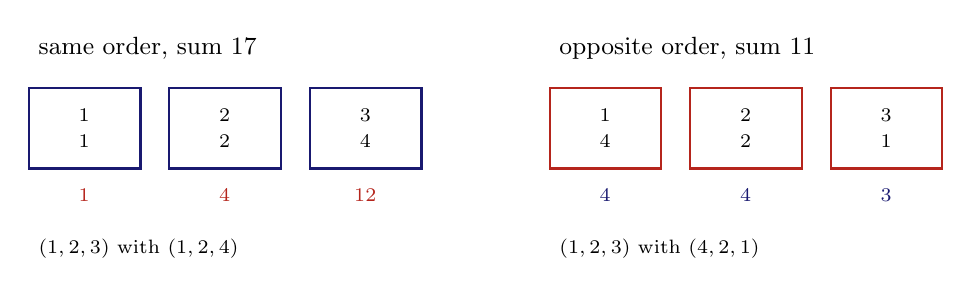
\begin{tikzpicture}[x=1.05cm,y=0.85cm,font=\scriptsize]
  \node[anchor=west,font=\small] at (0,3.15) {same order, sum $17$};
  \foreach \x/\va/\vb/\vp in {0/1/1/1, 1.7/2/2/4, 3.4/3/4/12} {
    \draw[MidnightBlue,thick] (\x,1.35) rectangle (\x+1.35,2.55);
    \node at (\x+0.67,2.15) {$\va$};
    \node at (\x+0.67,1.75) {$\vb$};
    \node[BrickRed] at (\x+0.67,0.95) {$\vp$};
  }
  \node[anchor=west,font=\small] at (6.3,3.15) {opposite order, sum $11$};
  \foreach \x/\va/\vb/\vp in {6.3/1/4/4, 8.0/2/2/4, 9.7/3/1/3} {
    \draw[BrickRed,thick] (\x,1.35) rectangle (\x+1.35,2.55);
    \node at (\x+0.67,2.15) {$\va$};
    \node at (\x+0.67,1.75) {$\vb$};
    \node[MidnightBlue] at (\x+0.67,0.95) {$\vp$};
  }
  \node[anchor=west] at (0,0.15) {$(1,2,3)$ with $(1,2,4)$};
  \node[anchor=west] at (6.3,0.15) {$(1,2,3)$ with $(4,2,1)$};
\end{tikzpicture}
